% abnTeX2: Modelo de Trabalho Academico (tese de doutorado, dissertacao de
% mestrado e trabalhos monograficos em geral) em conformidade com
% ABNT NBR 14724:2011: Informacao e documentacao - Trabalhos academicos -
% Apresentacao
% ------------------------------------------------------------------------

\documentclass[12pt,				% tamanho da fonte
	openright,			% capítulos começam em pág ímpar (insere página vazia caso preciso)
	oneside,			% twoside = para impressão em verso e anverso. Oposto a oneside
	a4paper,			% tamanho do papel. 
	% -- opções da classe abntex2 --
	%chapter=TITLE,		% títulos de capítulos convertidos em letras maiúsculas
	%section=TITLE,		% títulos de seções convertidos em letras maiúsculas
	%subsection=TITLE,	% títulos de subseções convertidos em letras maiúsculas
	%subsubsection=TITLE,% títulos de subsubseções convertidos em letras maiúsculas
	% -- opções do pacote babel --
	english,			% idioma adicional para hifenização
	brazil				% o último idioma é o principal do documento
	]{abntex2}

% ---
% Pacotes básicos 
% ---
\usepackage[T1]{fontenc}		% Selecao de codigos de fonte.
\usepackage[utf8]{inputenc}		% Codificacao do documento (conversão automática dos acentos)
\usepackage{lmodern}			% Usa a fonte Latin Modern			
\usepackage{cmap}				% Mapear caracteres especiais no PDF - tcc cartrac
\usepackage{lastpage}			% Usado pela Ficha catalográfica
\usepackage{indentfirst}		% Indenta o primeiro parágrafo de cada seção.
\usepackage{color}				% Controle das cores
\usepackage{graphicx}			% Inclusão de gráficos
\usepackage{microtype} 			% para melhorias de justificação
% ---	
% \usepackage{lipsum}				% para geração de dummy text
\usepackage{todonotes} 
\usepackage{url} 
% ---
% Pacotes de citações
% ---
%\usepackage[brazilian,hyperpageref]{backref}	 % Paginas com as citações na bibl
\usepackage[alf]{abntex2cite}	% Citações padrão ABNT

% --- 
% CONFIGURAÇÕES DE PACOTES
% --- 

% ---
% Configurações do pacote backref
% Usado sem a opção hyperpageref de backref
%\renewcommand{\backrefpagesname}{Citado na(s) página(s):~}
%% Texto padrão antes do número das páginas
%\renewcommand{\backref}{}
%% Define os textos da citação
%\renewcommand*{\backrefalt}[4]{
%	\ifcase #1 %
%		Nenhuma citação no texto.%
%	\or
%		Citado na página #2.%
%	\else
%		Citado #1 vezes nas páginas #2.%
%	\fi}%
% ---

% ---
% Informações de dados para CAPA e FOLHA DE ROSTO
% ---
\titulo{Coletando dados de memória de máquinas virtuais em nuvem para análise forense - PCS5012 - 2016/1}
% baseada em redes definidas por software
\autor{Hamilton Fonte II}
\local{São Paulo}
\data{2016}
\instituicao{%
  Universidade de São Paulo
  \par
  Escola Politécnica
  \par
  Departamento de Engenharia de Computação e Sistemas Digitais}
\tipotrabalho{Plano de Pesquisa}
% O preambulo deve conter o tipo do trabalho, o objetivo, 
% o nome da instituição e a área de concentração 
% \preambulo{Tese apresentada ao Departamento de Engenharia de Computa\c{c}\~ ao e Sistemas Digitais da Escola Polit\'ecnica da Universidade de S\~ao Paulo para obten\c{c}\~ ao do T\'{i}tulo de Livre Docente.}
% ---

% ---
% Configurações de aparência do PDF final

% alterando o aspecto da cor azul
\definecolor{blue}{RGB}{41,5,195}

% informações do PDF
\makeatletter
\hypersetup{
     	%pagebackref=true,
		pdftitle={\@title}, 
		pdfauthor={\@author},
    	pdfsubject={\imprimirpreambulo},
	    pdfcreator={LaTeX with abnTeX2},
		pdfkeywords={abnt}{latex}{abntex}{abntex2}{trabalho acadêmico}, 
		colorlinks=true,       		% false: boxed links; true: colored links
    	linkcolor=blue,          	% color of internal links
    	citecolor=blue,        		% color of links to bibliography
    	filecolor=magenta,      		% color of file links
		urlcolor=blue,
		bookmarksdepth=4
}
\makeatother
% --- 

% --- 
% Espaçamentos entre linhas e parágrafos 
% --- 

% O tamanho do parágrafo é dado por:
\setlength{\parindent}{1.3cm}

% Controle do espaçamento entre um parágrafo e outro:
\setlength{\parskip}{0.2cm}  % tente também \onelineskip

% ---
% compila o indice
% ---
\makeindex
% ---

% ----
% Início do documento
% ----
\begin{document}

% Retira espaço extra obsoleto entre as frases.
\frenchspacing

% ----------------------------------------------------------
% ELEMENTOS PRÉ-TEXTUAIS
% ----------------------------------------------------------
% \pretextual

% Capa
\imprimircapa

% --- Folha de rosto
% (o * indica que haverá a ficha bibliográfica)
% \imprimirfolhaderosto*

% ---
% Inserir a ficha bibliografica

% Isto é um exemplo de Ficha Catalográfica, ou ``Dados internacionais de
% catalogação-na-publicação''. Você pode utilizar este modelo como referência. 
% Porém, provavelmente a biblioteca da sua universidade lhe fornecerá um PDF
% com a ficha catalográfica definitiva após a defesa do trabalho. Quando estiver
% com o documento, salve-o como PDF no diretório do seu projeto e substitua todo
% o conteúdo de implementação deste arquivo pelo comando abaixo:
%
% \begin{fichacatalografica}
%     \includepdf{fig_ficha_catalografica.pdf}
% \end{fichacatalografica}
%\begin{fichacatalografica}
%	\vspace*{\fill}					% Posição vertical
%	\hrule							% Linha horizontal
%	\begin{center}					% Minipage Centralizado
%	\begin{minipage}[c]{12.5cm}		% Largura
%	
%	\imprimirautor
%	
%	\hspace{0.5cm} \imprimirtitulo  / \imprimirautor. --
%	\imprimirlocal, \imprimirdata-
%	
%	\hspace{0.5cm} \pageref{LastPage} p. : \\ %il. (algumas color.) ; 30 cm.\\
%	
%	\hspace{0.5cm} \imprimirorientadorRotulo~\imprimirorientador\\
%	
%	\hspace{0.5cm}
%	\parbox[t]{\textwidth}{\imprimirtipotrabalho~--~\imprimirinstituicao,
%	\imprimirdata.}\\
%	
%	\hspace{0.5cm}
%		1. Plano de Pesquisa.
%		2. Modelo.
%		3. PCS5012.
%		I. Universidade de São Paulo. Escola Politécnica. Departamento de Engenharia
%de Computação e Sistemas Digitais
%		II. t.\\ 			
%	
%	\hspace{8.75cm} CDU 02:141:005.7\\
%	
%	\end{minipage}
%	\end{center}
%	\hrule
%\end{fichacatalografica}
% ---

\pagebreak
% ---
% Dedicatória
% ---
%\begin{dedicatoria}
%   \vspace*{\fill}
%   \flushright
%   \noindent
%   \textit{``por que?'' é a pergunta mais importante. } 
%   \vspace*{\fill}
%\end{dedicatoria}
% ---

% ---
% Agradecimentos
% ---
%\begin{agradecimentos}
%
%
%\end{agradecimentos}
% ---

% ---
% Epígrafe -- deveria ser relacionada a área do conhecimento
% ---
%\begin{epigrafe}
%
%\end{epigrafe}
% ---

% ---
% RESUMOS
% ---

% resumo em português
\setlength{\absparsep}{18pt} % ajusta o espaçamento dos parágrafos do resumo
\begin{resumo}
Esta pesquisa tenta demonstrar que as abordagens para a coleta de informações de memória volátil de máquinas em nuvem com o propósito de análise forense disponíveis hoje não 
lidam com as características elásticas, multi-inquilino, multi-jurisdição da nuvem e os requisitos jurídicos para as evidências de forma satisfatória. Espero comprovar através
da implementação de um arcabouço de coleta destas informações, que a solução para estes problemas está em uma mudança na abordagem da coleta e armazenamento 
da evidência. Tendo êxito daremos um passo para a solução dos dois maiores problemas hoje na forense em nuvem, volume de dados crescente e a pouca conformidade com requisitos jurídicos.

% \vspace{\onelineskip}
 
%\noindent 
%\textbf{Palavras-chaves}: 

\end{resumo}

% resumo em inglês
%\begin{resumo}[Abstract]
%\begin{otherlanguage*}{english}
%
% \vspace{\onelineskip}
%  \noindent 
%  \textbf{Key-words}: 
%  
% \end{otherlanguage*}
%\end{resumo}


% ---
% inserir lista de ilustrações
% ---
%\pdfbookmark[0]{\listfigurename}{lof}
%\listoffigures*
%\cleardoublepage
% ---

% ---
% inserir lista de tabelas
% ---
%\pdfbookmark[0]{\listtablename}{lot}
%\listoftables*
%\cleardoublepage
% ---

% ---
% inserir lista de abreviaturas e siglas
% ---
%\begin{siglas}
%   \item[USP]    Universidade de São Paulo
%\end{siglas}
% ---

%% ---
%% inserir lista de símbolos
%% ---
%\begin{simbolos}
%  \item[$ \Gamma $] Letra grega Gama
%  \item[$ \Lambda $] Lambda
%  \item[$ \zeta $] Letra grega minúscula zeta
%  \item[$ \in $] Pertence
%\end{simbolos}
%% ---

% ---
% inserir o sumario
% ---
%\pdfbookmark[0]{\contentsname}{toc}
%\tableofcontents*
%\cleardoublepage
% ---

% ----------------------------------------------------------
% ELEMENTOS TEXTUAIS
% ----------------------------------------------------------
\textual

%%%%%%%%%%%%%%%%%%%%%%%%%%%%%%%%%%%%%%%%%%%%%%%%%%%%%%
\chapter{Descrição do problema de pesquisa} \label{chap:intro}
%\input{chap/01-intro}
Forense digital é um conjunto de técnicas de coleta e análise de evidências geradas por computadores que tem por objetivos, entender a sequência de eventos que permitiu que um 
ataque ocorresse, impedir que a vulnerabilidade que tornou possível o ataque seja explorada novamente e apoiar os processos jurídicos que visam submeter os culpados as punições
previstas na lei \cite{Sang2013}. 
A forense digital cresceu a partir de técnicas usadas na forense tradicional. Começou de forma artesanal, passou por uma fase de adaptação aos requisitos legais até a era atual
de ferramental avançado de coleta e análise \cite{Charters2008}.

A utilização crescente de virtualização, ferramentas online e hospedagem em nuvem \cite{Amazon2016}, está criando dificuldades para a coleta de informações, análise e utilização 
em processos legais \cite{Sharma2012}. A funcionalidade de elasticidade de carga ofertada pelos provedores de nuvem por meio da qual infraestrutura pode ser 
alocada e desalocada dinamicamente, trouxe o problema da volatilidade dos dados nas máquinas virtuais. Com algumas ameaças que não deixam evidências em disco \cite{Rafique2013}, 
a memória de uma máquina virtual despejada de um pool e seus recursos liberados seria para sempre perdida e com ela evidências importantes. O simples armazenamento do conteúdo 
da memória não satisfaz o requisito jurídico de se repetir o processo e conseguir os mesmos resultados. A abordagem de armazenar constantemente todas as alterações da
memória não contribui para a solução do crescente backlog de dados que os investigadores tem para analizar \cite{Quick2014}. 

O ferramental forense disponível hoje está pouco adaptado a desafios trazidos pela nuvem \cite{Dykstra2012a}, focam em completude e poucos geram evidências aceitáveis em um 
processo jurídico \cite{Reichert2015}. A cadeia de custódia, um processo de coleta e armazenamento de evidências que visa garantir que a evidência não foi alterada, destruída 
ou manipulada por pessoas não autorizadas, é pouco abordada nas soluções existentes hoje. 

A solução destes problemas passa pela confirmação das seguintes hipóteses

\begin{enumerate}
 \item \textbf{É possível conseguir o mesmo resultado da coleta mesmo se a máquina e o processo de origem não existirem mais}: Esta hipótese esta associada a necessidade jurídica de se 
 repetir o processo de coleta e conseguir os mesmos resultados em um cenário onde as evidências de um ataque estavam na memória de uma máquina virtual que foi despejada do pool e
 teve seus recursos liberados.
 Como a maioria das soluções de coleta hoje se baseiam em isolamento da máquina virtual afetada ou no armazenamento de informação de log, comprovar esta hipótese nos dá
 a oportunidade de fechar uma forma de se conseguir impunidade em crimes cometidos na nuvem.
 \item \textbf{Não é necessário todo o histórico de alterações da memória nem a cópia bit a bit da mesma para a análise do incidente}: Esta hipótese esta associada ao crescente
 volume de informações que precisam ser analisadas pelos investigadores forenses. Em 2014 a média era de 6 a 12 meses de backlog \cite{Quick2014}. A confirmação desta hipótese
 envolve a aceitação de uma mudança no paradigma de coleta de informações forenses de 'completude' para 'a coleta do necessário'.
\end{enumerate}

Esta pesquisa tenta resolver os 2 maiores problemas da forense em nuvem hoje sugerindo uma mudança no paradigma da coleta de informações de memória das máquinas. Os desafios apresentados
neste capítulo mostram que as abordagens atuais estão se esgotando e acompanhar a evolução da nuvem requer uma mudança nos procedimentos de coleta.

\chapter{Objetivos} \label{chap:obj}
A aceitabilidade de evidências resultantes do trabalho de peritos é regulada por um conjunto de regras da lei Norte-Americana. Deste conjunto de leis derivou-se 3 requisitos que
a evidência coletada de nuvem precisa se submeter, são eles: A obrigatoriedade em garantir que as provas não foram comprometidas ou alteradas durante o processo de coleta, o processo
de coleta ser capaz de gerar as mesmas evidências quando executado novamente por outra pessoa e por fim conhecer sua taxa de erro. A maioria das pesquisas relacionadas a coleta de 
informações tem viés técnico e poucos lidam com os aspectos legais relacionados a coleta de informações. Sendo assim temos:\\

\noindent \textbf{Objetivo geral}: Provar que é possível coletar dados de memória de processos em máquinas na nuvem de modo que estes atendam
aos 3 requisitos legais mencionados anteriormente. \\

\noindent \textbf{Objetivos específicos}:
\begin{enumerate}
 \item Conseguir reproduzir o processo de coleta mesmo se a máquina de onde se originaram os dados tiver sido despejada e seus recursos liberados.
 \item Descobrir o mínimo de informação necessária antes do incidente de modo a viabilizar a análise.
 \item Conseguir realizar a coleta sem violar jurisdição e privacidade de usuários não relacionados a investigação mantendo a cadeia de custódia.
 \item Conhecer a taxa de erro do processo.
\end{enumerate}

\chapter{Método} \label{chap:metodo}

\begin{flushleft}Para atingir os objetivos:\end{flushleft} 

\begin{itemize}
 \item \textbf{Conseguir reproduzir o processo de coleta mesmo se a máquina de onde se originaram os dados tiver sido despejada e seus recursos liberados}
 \item \textbf{Conhecer a taxa de erro do processo} 
\end{itemize}

\begin{flushleft}é preciso construir os seguintes artefatos:\end{flushleft}

\begin{enumerate}
 \item Construir uma máquina virtual e desenvolver uma aplicação que serão o alvo da coleta. A máquina virtual será construída usando programas de gerenciamento 
 de configuração como Puppet \cite{Wikipedia2015} ou Vagrant\cite{Wikipedia2016} e a aplicação será instalada na máquina virtual usando um programa automatizador de 
 instalação baseado em conteiner como o Docker \cite{Wikipedia2016a}. A aplicação será uma página web dinâmica hospedada em um servidor Nginx \cite{Wikipedia2015a} na
 máquina alvo que responde um HTML contendo a palavra 'ACK' para qualquer requisição.
 
 \item Desenvolver uma ameaça simples que altera a memória da aplicação alvo da coleta.
 
 \item Desenvolver uma aplicação de coleta de informações de memória em nuvem de modo que se consiga relacionar a mesma a sua origem e que o resultado seja o mesmo.
 
 Com os artefatos construídos acima conduzir o experimento:

\begin{enumerate}
 \item Criar a máquina virtual.
 \item Executar a aplicação de coleta de evidência.
 \item Aplicar a ameaça.
 \item Despejar a máquina virtual e liberar seus recursos.
 \item Identificar e guardar a evidência.
 \item Repetir os passos anteriores.
\end{enumerate}

\textbf{A medição}: Estamos interessados em avaliar o quão idênticas são as evidências coletadas no processo. É esperado que haja alguma diferença pela natureza dinâmica da memória. 

Formalmente não há um limite máximo ou mínimo de erro aceitável no processo de coleta. No procedimento jurídico, a evidência é anexada junto com a descrição do método 
de coleta e o erro associado onde então, caso uma das partes entenda ser necessário, pode ser contestada. Assim sendo a medição do erro da coleta será feita comparando 
a evidência coletada com as coletadas anteriormente. Esta comparação será feita bit a bit e o resultado será o cálculo da \% de bits diferentes entre as duas coletas. 
Cada nova evidência gerada será comparada com as coletas anteriores e a média das comparações será a \textbf{taxa de erro do processo de coleta}.

\end{enumerate}

\begin{flushleft}Para atingir os objetivos: \end{flushleft} 

\begin{itemize}
 \item \textbf{Descobrir o mínimo de informação necessária antes do incidente de modo a viabilizar a análise}
 \item \textbf{Conseguir realizar a coleta sem violar jurisdição e privacidade de usuários não relacionados a investigação mantendo a cadeia de custódia} 
\end{itemize}

\begin{flushleft}é preciso construir o seguinte artefato:\end{flushleft}

\begin{enumerate}

\item O diagrama de um arcabouço para transportar a evidência da máquina virtual alvo construida para o experimento anterior até um local de armazenamento fora da nuvem. Este 
transporte será realizado via TLS e o ambiente de destino da evidência terá o acesso controlado por chave privada.

\textbf{A validação do arcabouço}: O trabalho do perito é regido por uma norma que trata, entre outras coisas, dos procedimentos que devem ser executados para coleta. Esta norma no Brasil é o 
Código de Processo Penal que foi instituído pelo decreto lei N\textsuperscript{\underline{o}} 3689 de 3 de outubro de 1941. O Código Penal Brasileiro em sua Parte Especial 
tipifica uma série de crimes digitais mas assim como o Código de Processo Penal possuem brechas \cite{Do2014} pois não evoluíram tão rápido quanto a tecnologia. Com isso, 
aferir se a solução atende aos objetivos mencionados depende de opinião de peritos assim, temos as seguintes ações:

\end{enumerate}

\begin{itemize}

\item Entrevistar peritos forenses, apresentá-los o arcabouço de armazenamento e coletar opiniões sobre a sua aceitabilidade.

\item Entrevistar peritos forenses, apresentá-los a taxa de erro do processo e coletar opiniões sobre a sua aceitabilidade.

\item Entrevistar novamente peritos forenses, apresentá-los a estratégia de armazenamento mínimo e coletar opiniões sobre a sua aceitabilidade. 

\end{itemize}

\chapter{Revisão bibliográfica} \label{chap:related}
A revisão bibliográfica focou nos seguintes conceitos da coleta de informações forenses em nuvem:

\begin{itemize}
 \item Acessar e coletar as informações, de memória ou não, das máquinas virtuais em nuvem.
 \item Conformidade com os seguintes requisitos jurídicos: 
 \begin{itemize}
  \item Reproduzir o processo com os mesmos resultados e conhecer a taxa de erro.
  \item Não violar privacidade de outros usuários de nuvem ou jurisdição de outros países.
  \item Garantir a cadeia de custódia da evidência.
 \end{itemize}
\end{itemize}

Com a revisão constatou-se que, referente a coleta de informações a maioria dos trabalhos mais importantes na área \cite{Reichert2015}, \cite{Poisel2013}, \cite{Dykstra2013}, 
\cite{George2012} e \cite{Sang2013} focam em coleta reativa, isto é, ela acontece apenas após a ameaça ser detectada. Podem acontecer por acionamento manual ou integrada a um 
mecanismo de detecção de ameaça. Em casos de memória volátil, esta forma de coleta de informação não consegue descrever como era a memória antes do ataque. Esta capacidade é
necessária para viabilizar a abordagem de coletar o mínimo necessário para realizar a investigação e apoiar o processo jurídico. A única proposta encontrada que leva esta 
necessidade em consideração é \cite{Dezfouli2012} mas propõe que o dado seja armazenado no próprio dispositivo o que pode levar a perda de informações importantes caso a 
máquina virtual seja despejada do pool e seus recursos liberados.

Ainda na coleta de informações, \cite{Reichert2015}, \cite{George2012} sugerem a abordagem de forense ao vivo onde os dados são coletados com o sistema rodando enquanto 
\cite{Poisel2013}, \cite{Dykstra2013}, \cite{Sang2013} adotam a estratégia de isolar e/ou parar a máquina virtual e em seguida executar o processo de coleta. Nos dois casos, 
nenhum dos autores cobre o cenário onde a máquina virtual é despejada do pool e os recursos são liberados. Analisando cuidadosamente as propostas de \cite{Poisel2013}, parece que é possível
cobrir o cenário mencionado anteriormente mas ele não dá detalhes da implementação suficientes para termos certeza.

Referente aos requisitos legais, nenhuma das propostas consegue reproduzir os mesmos resultados ao repetir o processo no cenário em que uma máquina virtual é despejada da nuvem e seus 
recursos liberados. Analisando cuidadosamente a proposta de \cite{George2012} parece que é possível mas o autor não dá detalhes de implementação suficientes para termos certeza.

No armazenamento das informações coletadas, \cite{Reichert2015}, \cite{George2012}, \cite{Poisel2013} e \cite{Dykstra2013} usam estratégia de armazenamento fora da nuvem para 
resolver o problema de jurisdição e violação de privacidade de outros usuários no processo da coleta \cite{Sang2013} e um caso específico de \cite{George2012} dependem de 
cooperação do provedor de serviços de nuvem para conseguir as informações necessárias à investigação. Depender do provedor de serviços de nuvem é uma estratégia fraca pois o foco
deles é garantir a continuidade do serviço não a coleta de evidências. 

Na garantia da cadeia de custódia apenas \cite{Sang2013} tenta resolver a questão mas toma cuidados apenas para  garantir que a evidência não foi destruída ou alterada. 
Ele faz isso através de cálculo de hashing mas não explica como impede o acesso não autorizado à evidência. As propostas dos outros autores estão focadas apenas no 
aspecto técnico da coleta.

\chapter{Resultados esperados} \label{chap:result}
O primeiro resultado esperado é um arcabouço que consiga coletar informações de memória de processos de máquinas na nuvem e armazená-las em um local físico conhecido.
Este armazenamento deve garantir a integridade e a confidencialidade da evidência. O volume de informações armazenadas será o suficiente para diferenciar o sistema antes 
e depois que a ameaça foi detectada. A utilização deste arcabouço sob as mesmas condições deve gerar um conjunto idêntico de evidências. Com isso, será possível fechar 
uma das formas de impunidade para os atos ilícitos em nuvem e contribuir para a diminuição do backlog de investigação.

\chapter{Cronograma} \label{chap:cronograma}

O plano de trabalho é descrito pelas seguintes atividades e organizado de acordo com o apresentado na Figura 1. Este cronograma pode sofrer alterações ao longo da realização da
pesquisa.

\begin{itemize}
 \item Revisão bibliográfica
 \item Acompanhamento do estado da arte
 \item Estudo das aplicações baseadas em container
 \item Implementação da receita para a máquina virtual
 \item Implementação da aplicação de coleta
 \item Implementação da ameaça
 \item Execução do experimento de coleta
 \item Analise dos resultados e ajustes na aplicação de coleta
 \item Documentação do arcabouço
 \item Entrevista com peritos
 \item Ajuste no arcabouço
 \item Escrita e defesa de tese.
\end{itemize}

\begin{figure}
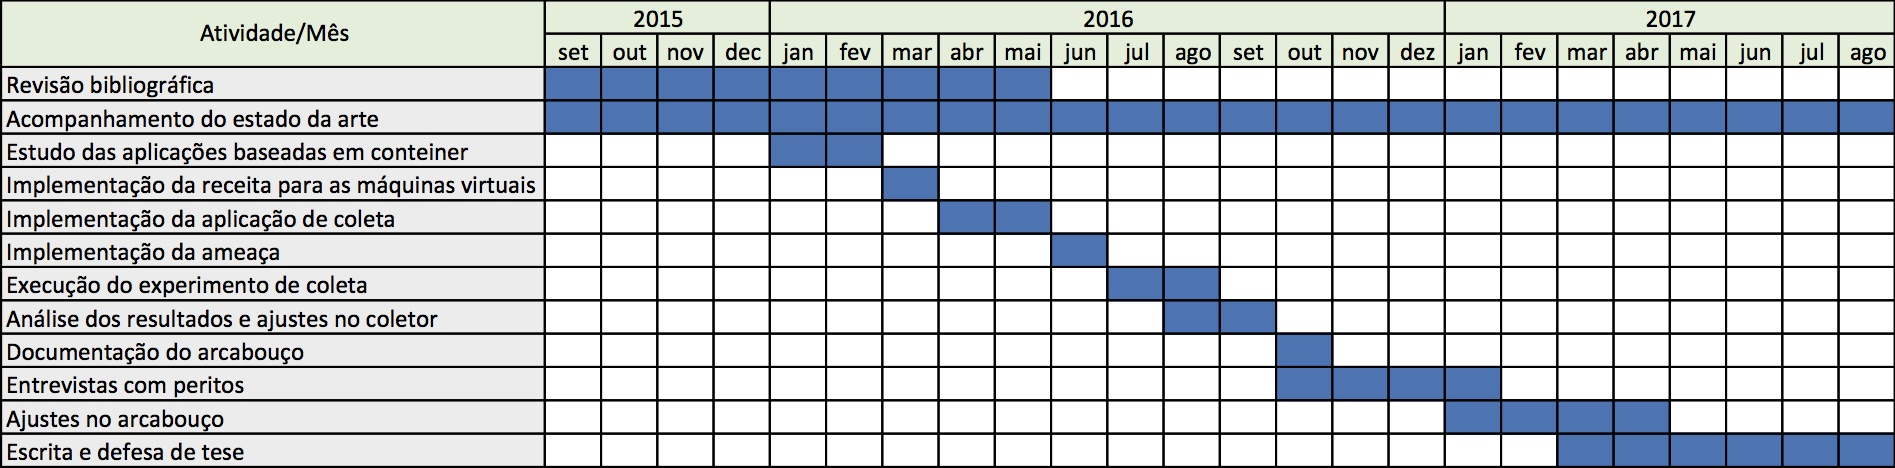
\includegraphics[keepaspectratio, scale=0.26]{Cronograma}
\caption{Fonte: Autor}
\end{figure}

\bibliography{abntex2-modelo-references}

% ----------------------------------------------------------
% ELEMENTOS PÓS-TEXTUAIS
% ----------------------------------------------------------
\postextual

% ----------------------------------------------------------
% Referências bibliográficas
% ----------------------------------------------------------
%  \bibliography{•}

%---------------------------------------------------------------------
% INDICE REMISSIVO
%---------------------------------------------------------------------
\begin{comment}
\printindex
\end{comment}

%%%%%%%%%%%%%%%%%%%%%%%%%%%
\end{document}
